\chapter{Results}
% (2-4 pages)

\section{Final User Interface}
%-------------------------------------------%
As previously mentioned, we used Tkinter for creating the interface, with some code generation from Page, a drag-and-drop Python GUI program.  Our original interface consisted simply of a setup window for choosing parameters to send to the Driving Assistant.  This was because we were constantly changing the parameters during development, and since they were hard coded, we would have to go back and change the code each time.  The following are parameters changeable in the interface:

\paragraph{Monitor ID:} This selects which monitor to feed frames. The default values are $0, 1, and~ 2$. For the typical dual-monitor setup, 0 is both, whereas 1 and 2 are the other individual monitors.

\paragraph{Custom Window Size:} If the Set Custom Window Size button is not checked, then the frame size will default to the size of the entire monitor that's feeding the visual stream. If it's checked, this allows the user to enter a custom size (a smaller window size results in better performance).

\paragraph{Top/Left Offset:} By default, the visual stream will be feeding from the very top left corner on the monitor, even with a custom smaller window size. Adding an offset allows the user to change what part of the screen is being fed to the visual feed.

\paragraph{Enable Object Detection:} Toggles whether to run object detection.

\paragraph{Enable Lane Detection:} Toggles whether lane detection runs -- will significantly decrease FPS.

\paragraph{Enable Object Visualization:} Toggles whether to visualize objects -- will decrease FPS.

\paragraph{Enable Lane Visualization:} Toggles whether to visualize lanes -- will decrease FPS.

\paragraph{Diagnostic Mode:} Toggles whether to run in diagnostic mode. Every time the run method is called, a frame is exported before and after the object/lane detection. The values of the threat dictionary are added to a CSV that lists the threat dictionary results from each frame for testing purposes.

\paragraph{CNN:} There are three options for changing the feature identifier model. The default is Resnet101, which gives us the best hardware performance. NAS is a more accurate model, however its performance is slower. Inception-Resnet is a compromise between the two, however we did not find a measurable performance benefit.

\paragraph{Dataset:}There are two options: Coco and Kitti. Coco is an American trained dataset, with more classes, so this is the default option. Kitti has fewer classes, and was trained in Europe.

\paragraph{Threshold:} This controls the confidence threshold cutoff for detected objects. Any object detected with a confidence below the set threshold will not be displayed onscreen. The default value is 85\%.


\begin{figure}[h!]
	\centering
    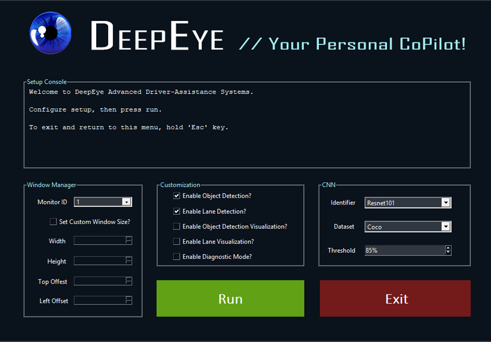
\includegraphics[width=1.0 \linewidth]{main-interface.png}
    \caption{Main Interface}
\end{figure}

After the first iteration, we added a text box to display text normally output in a separate terminal window, to make it cleaner and let the user know it's running, as it can take a while to load.  After setting the parameters, the user can press the "Run" button to start the program.  Once it starts, the frames containing the setup widgets are hidden behind the new runtime interface.  While not ideal, this was done to bypass limitations related to Tkinter, which will be further discussed below. \\

\begin{figure}[h!]
	\centering
    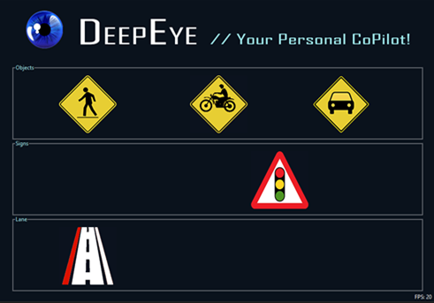
\includegraphics[width=1.0 \linewidth]{warning-interface.png}
    \caption{Dashboard (Warning Interface)}
\end{figure}

In the runtime interface, there are three frames: One for objects (vehicles, bikes, and pedestrians), one for signs (stop signs and traffic lights), and one for lane detection.  In each frame, an icon will show up for each detected object.  In the lane detection frame, an icon will display, informing the driver the position of the lane they are in.  If no lane is detected, a separate icon displays.  When a collision threat is detected, a warning icon is displayed while all other icons are cleared from the interface in order to bring greater attention to this. An audible beep is also played.  

While the program is running, the user can press "Escape" to stop the program and return to the setup menu.  There they can either edit parameters and run again, or press "Exit" to quit the program altogether.  

%-------------------------------------------%

\pagebreak


\section{Analytical/Testing Results}
%-------------------------------------------%

\paragraph{Summary:}  While running in diagnostic mode, two screenshots are taken every several frames; one before the object and lane detection runs, and one after, which shows the objects and lane detected.  When the screenshots are taken, the values of the threat dictionary are added to a CSV with the corresponding frame. A value of (0) means the threat is not present, while a (1) means it was detected.  We made a copy of this data frame, removed the generated values, and then manually added them in by going through each frame and determining if the threat was present to represent the ground-truth.  We then compared the original data frame to the one we filled out.

\paragraph{Overall Performance:} We ran the diagnostic mode on roughly an hour's worth of driving videos. Particularly, (26) minutes of dash-cam streams captured using a dash-camera mounted on the front windshield of the car, and (30) minutes of first-person view of us driving in GTA-V. Then, we ran our testing script to figure out our ratio for true positive/negative predictions (when the system was correct) compared to false predictions. Lastly, we designed a rating system on a (0-100 scale) to describe the accuracy of our system -- meaning how the system is doing in terms of making the right predictions. Comparing the data frame that was automatically generated by our system to the ground-truth data frame showed that the our system is $92\%$ accurate in various situations such as (crowded areas, tunnels, and highways) on the dash-cam streams, while being $87\%$ accurate in various weather/lighting conditions controlled within a virtual environment (GTA-V) as shown in the tables below: 


\begin{figure}[h!]
  \centering
  \subfigure[]
  {%
    \label{fig:Overall Performance - DashCam}%
    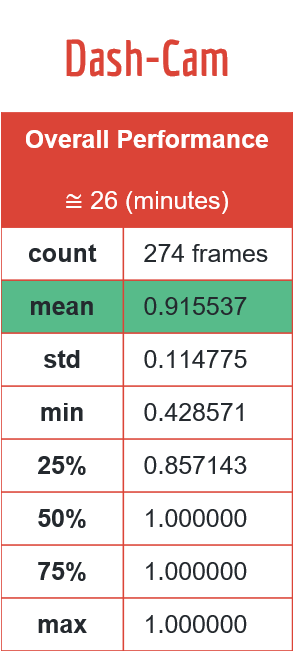
\includegraphics[width=.25 \linewidth]{dashcam-avg.png}
  }%
  \qquad 
  \subfigure[]
  {%
    \label{fig:Overall Performance - GTAV}%
    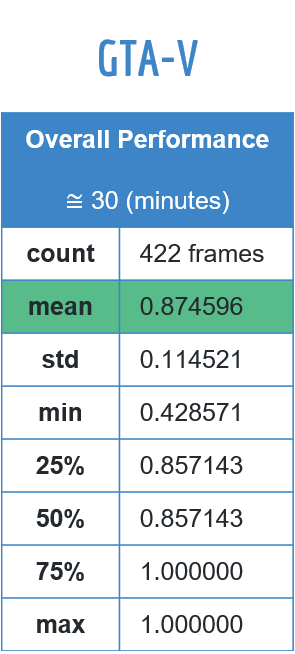
\includegraphics[width=.25 \linewidth]{gtav-avg.png}
  }%
  \caption{Overall Performance}
\end{figure}


\paragraph{Performance By Individual Target:} To further investigate our results, we modified our testing script to include a rating score for each feature in the system. As expected, most scores indicated that our system is performing fairly well, with the exception of off-lane detection and collision detection. Notably, research in the last few years has showed that vision-based solutions for both off-lane detection and collision detection are not ideal. There are several approaches that would achieve better results such as sensory-based system (LIDAR, RADAR, etc). The resulting scores for each feature are stated in the tables below: 

\begin{figure}[h!]
  \centering
  \subfigure[]
  {%
    \label{fig:Individual Performance - DashCam}%
    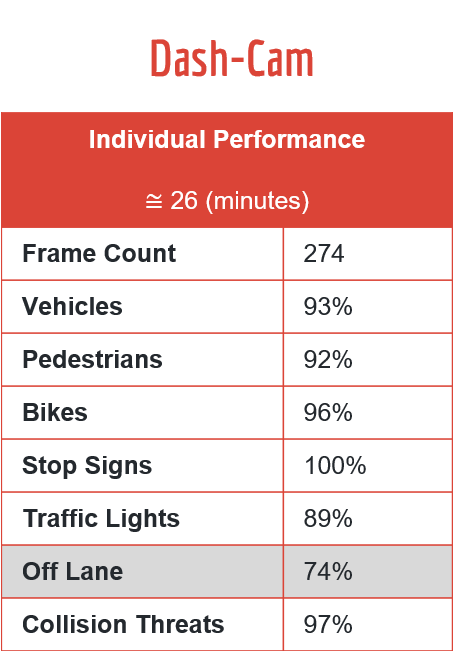
\includegraphics[width=.36 \linewidth]{dashcam-scores.png}
  }%
  \qquad
  \subfigure[]
  {%
    \label{fig:Individual Performance - GTAV}%
    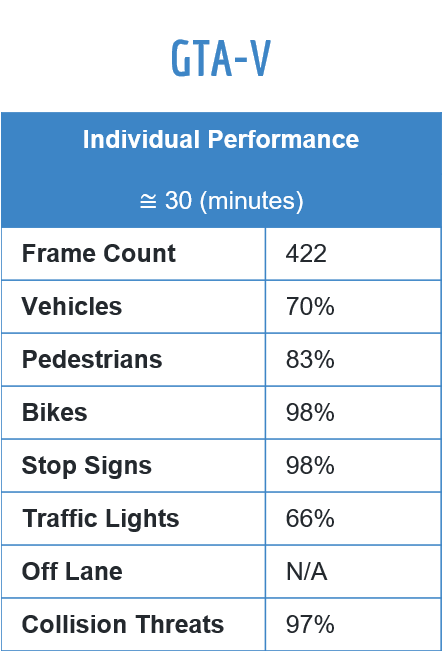
\includegraphics[width=.35 \linewidth]{gtav-scores.png}
  }%
  \caption{Individual Performance}
\end{figure}
\par 

%-------------------------------------------%

